\chapter{User Interface}

\section{User Interface Draft 1}
	\label{uiDrafts} 

	\begin{figure}[H]
		\centering
		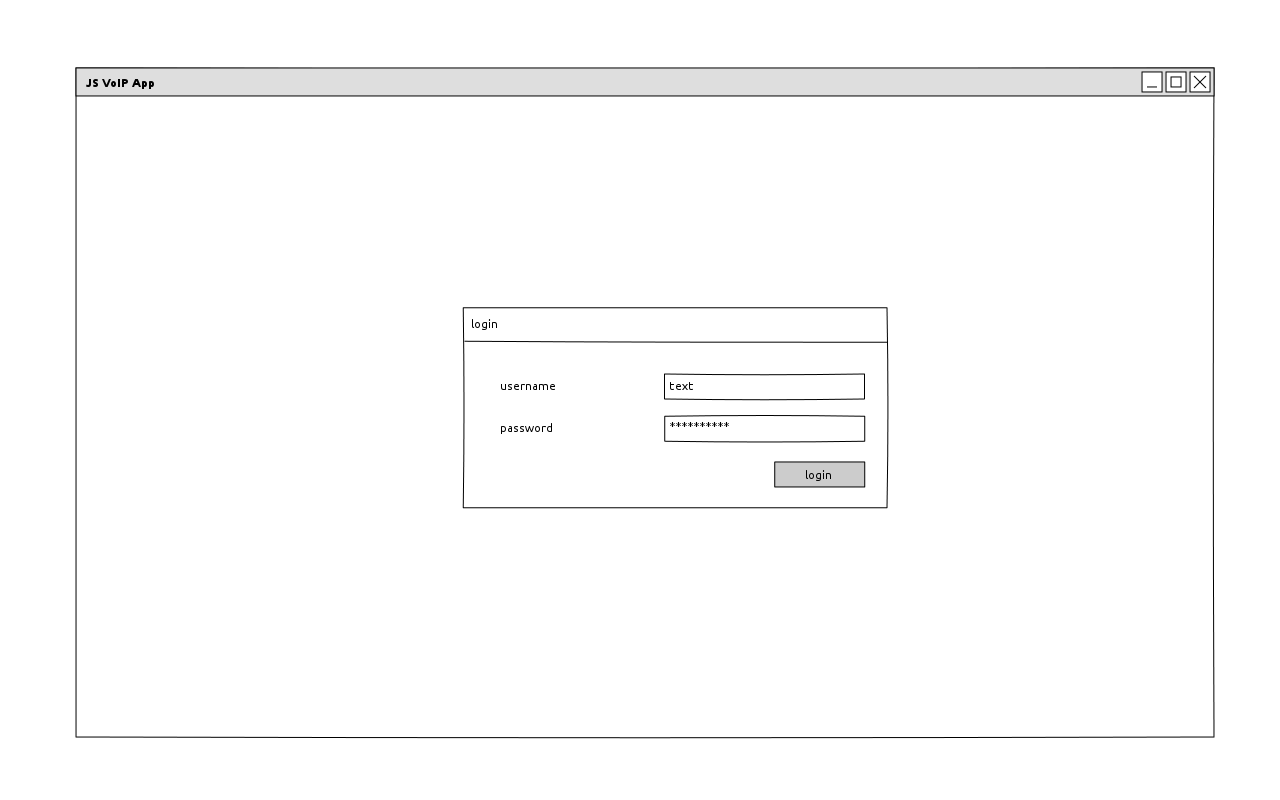
\includegraphics[height=0.3\textheight]{../ui/img/uiDraft1/login_page.png}
		\caption[Login screen draft1]{Über den Login Screen loggen sich Benutzer ein.}
		\label{login screen}
	\end{figure}
	\begin{figure}[H]
		\centering
		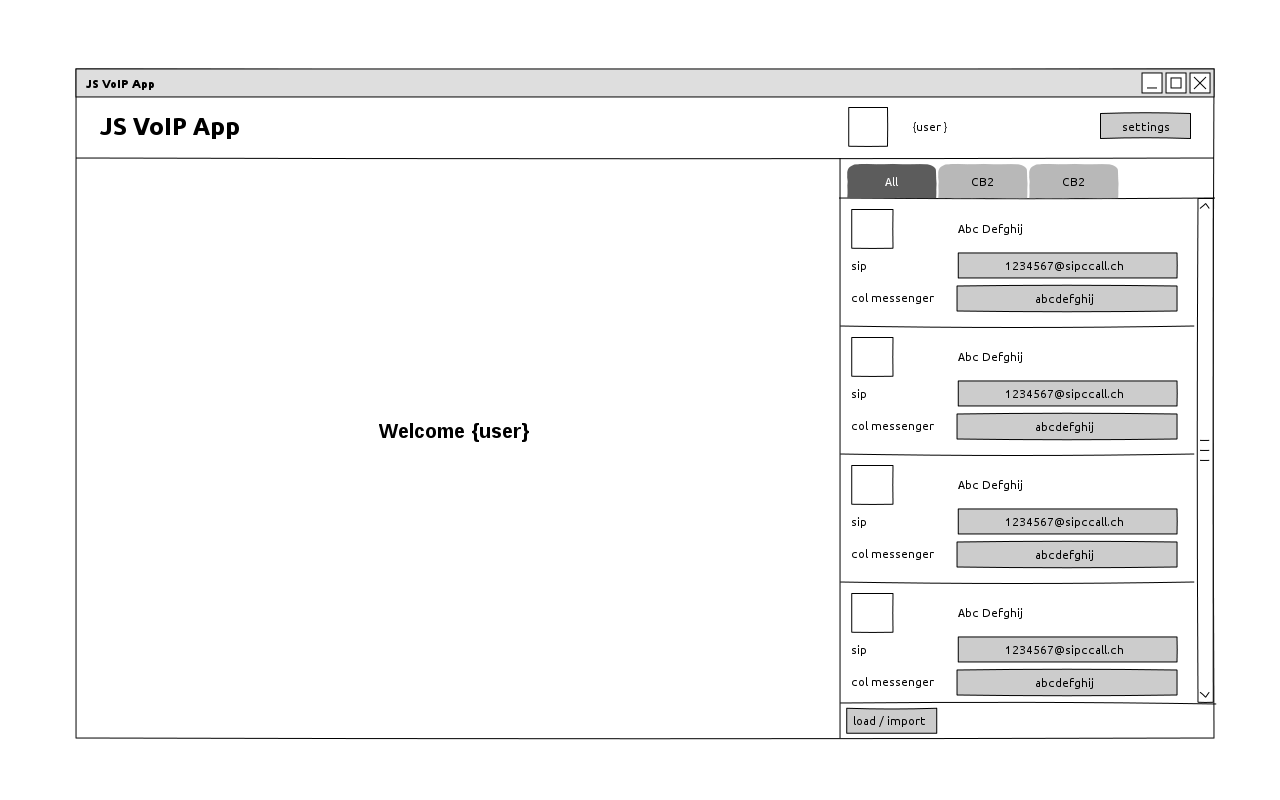
\includegraphics[height=0.3\textheight]{../ui/img/uiDraft1/main_view.png}
		\caption[Main screen draft1]{In der Hauptansicht hat der Benutzer Zugriff auf das Adressbuch.}
		\label{main screen}
	\end{figure}
	\begin{figure}[H]
		\centering
		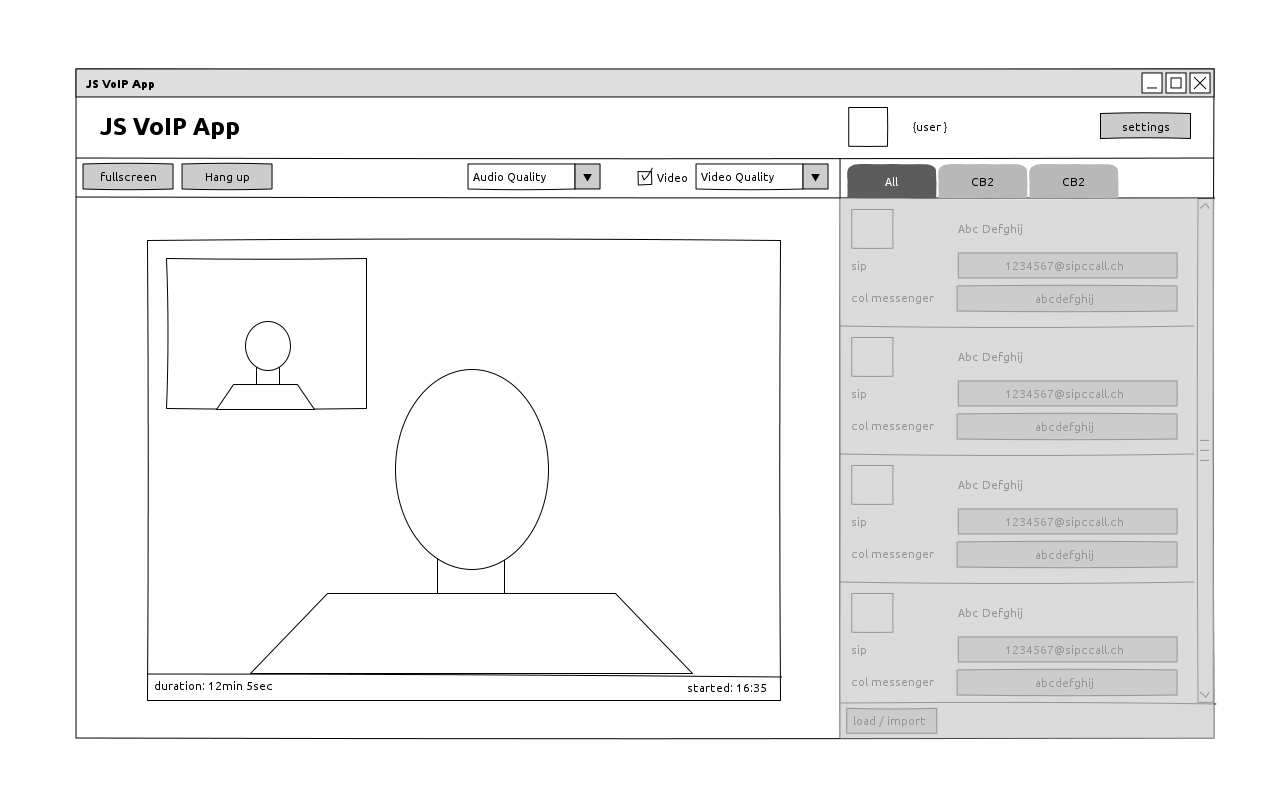
\includegraphics[height=0.4\textheight]{../ui/img/uiDraft1/call_view.png}
		\caption[Phone screen draft1]{Ruft der Benutzer einen Kontakt an, so wird das Video in der Hauptansicht eingeblendet und die Kontakte werden inaktiv.}
		\label{call screen}
	\end{figure}
	\begin{figure}[H]
		\centering
		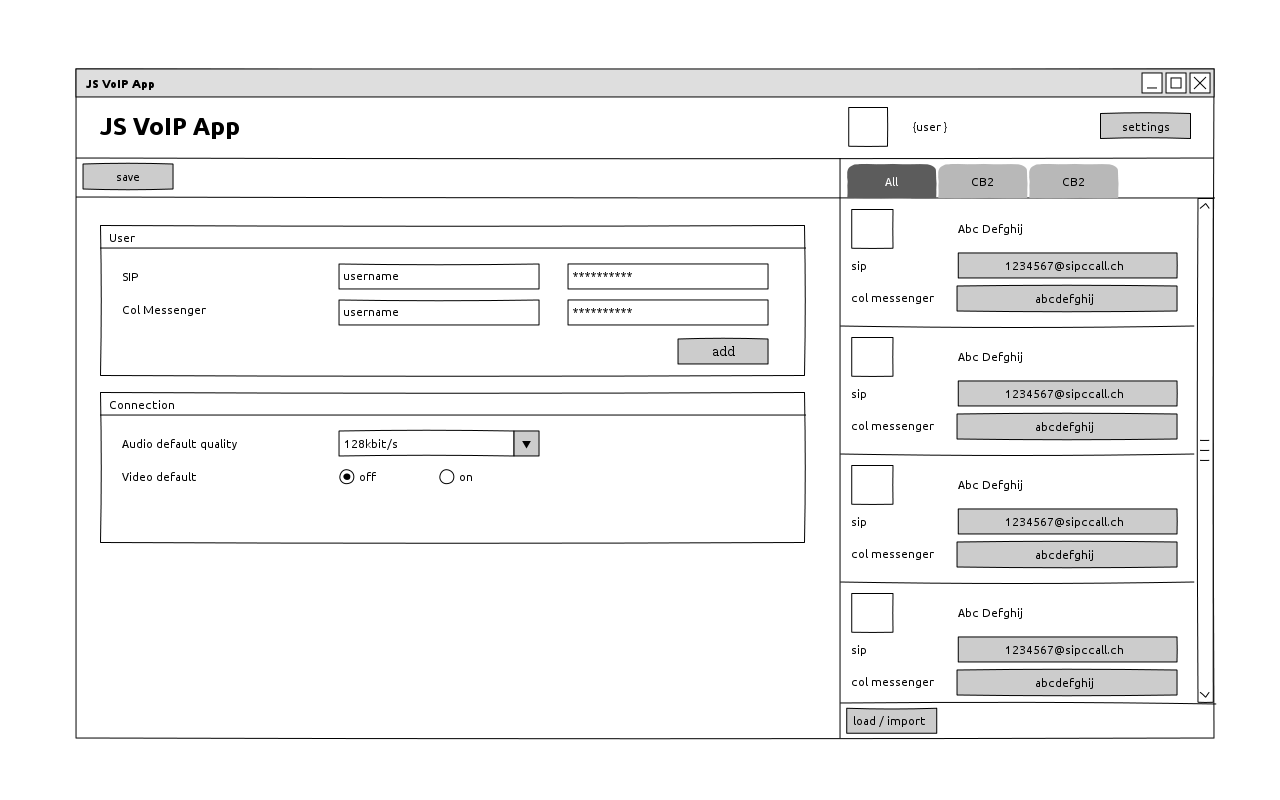
\includegraphics[height=0.4\textheight]{../ui/img/uiDraft1/settings_view.png}
		\caption[Settings screen draft1]{Über die Settings kann der Bentzer Einstellungen verändern.}
		\label{settings screen}
	\end{figure}
	
	
\section{User Interface Draft 2}
	Das UI2 folgt dem Prinzip ``Mobile First"'.
	\begin{figure}[H]
		\centering
		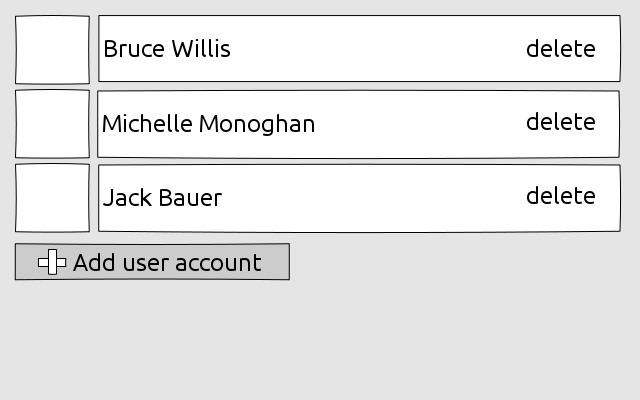
\includegraphics[height=0.35\textheight]{../ui/img/uiDraft2/UserView-selectUser.png}
		\caption[Accound screen draft2]{Benutzer Verwaltung und Login Screen. Durch klick auf einen Benutzer kann sich der Benutzer mit dessen Konto anmelden.}
		\label{login screen}
	\end{figure}
	\begin{figure}[H]
		\centering
		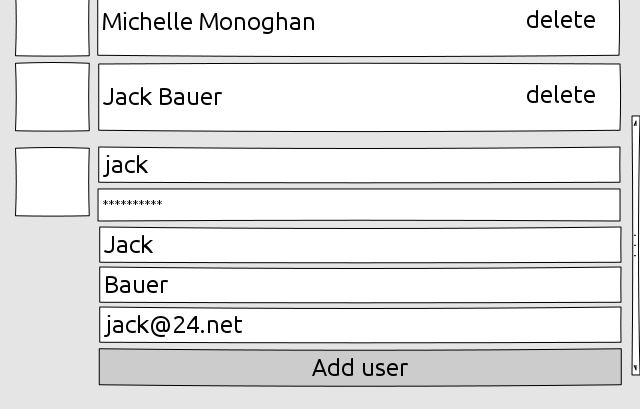
\includegraphics[height=0.35\textheight]{../ui/img/uiDraft2/UserView-addUser.png}
		\caption[Account management Screen draft2]{Die Benutzerverwaltung erlaubt es dem benutzer auch gleich einen neuen Bentzer zu erfassen.}
		\label{user management screen}
	\end{figure}
		\begin{figure}[H]
		\centering
		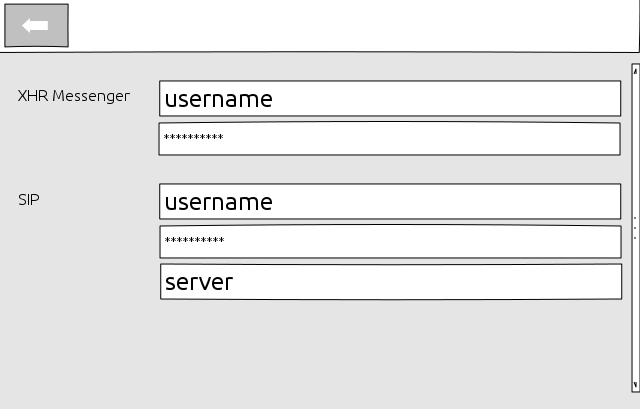
\includegraphics[height=0.4\textheight]{../ui/img/uiDraft2/UserView-addChannel.png}
		\caption[Channel edit screen draft2]{Die Bentzerverwaltung ermöglicht dem Benutzer das verwalten der verfügbaren Channel Accounts.}
		\label{user management screen}
	\end{figure}
	\begin{figure}[H]
		\centering
		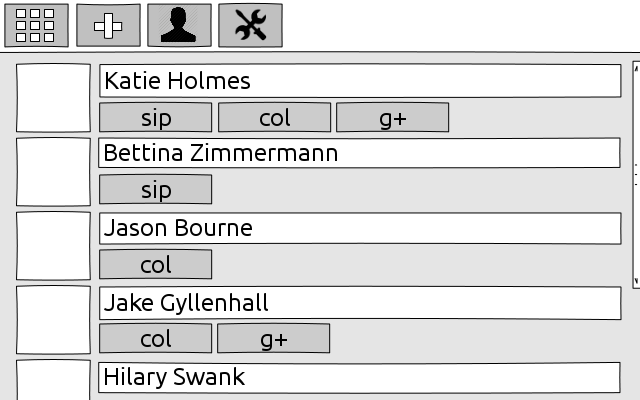
\includegraphics[height=0.4\textheight]{../ui/img/uiDraft2/ContactbookView.png}
		\caption[Contactbook screen draft2]{Adressbuch: Von hier aus ruft der Benutzer seine Kontakte an. Die verschiedenen Adressbücher sind über das Listensymbol erreichbar.}
		\label{contactbook screen}
	\end{figure}
	\begin{figure}[H]
		\centering
		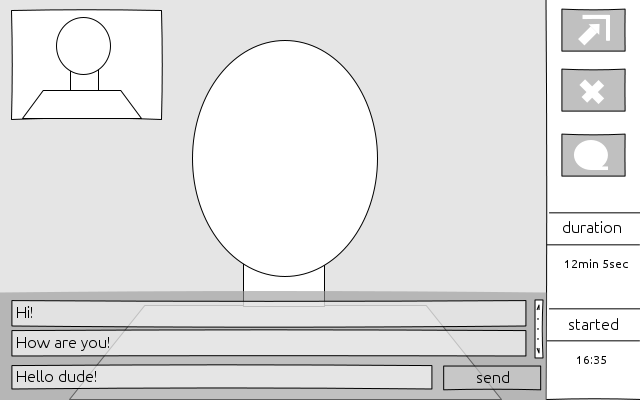
\includegraphics[height=0.4\textheight]{../ui/img/uiDraft2/PhoneViewWithMessenger.png}
		\caption[Call screen draft2]{Phone View: Nebst dem Video sieht der Benutzer elementare Informationen über den Anruf.}
		\label{settings screen}
	\end{figure}
	\begin{figure}[H]
		\centering
		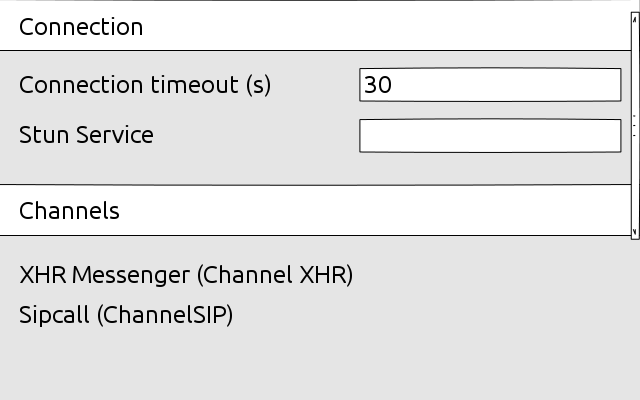
\includegraphics[height=0.4\textheight]{../ui/img/uiDraft2/SettingsView.png}
		\caption[Settings screen draft2]{In den Settings kann der Benutzer Konfiguration und Channels einsehen.}
		\label{settings screen}
	\end{figure}
	
\section{Finales User Interface}
	\begin{figure}[H]
		\centering
		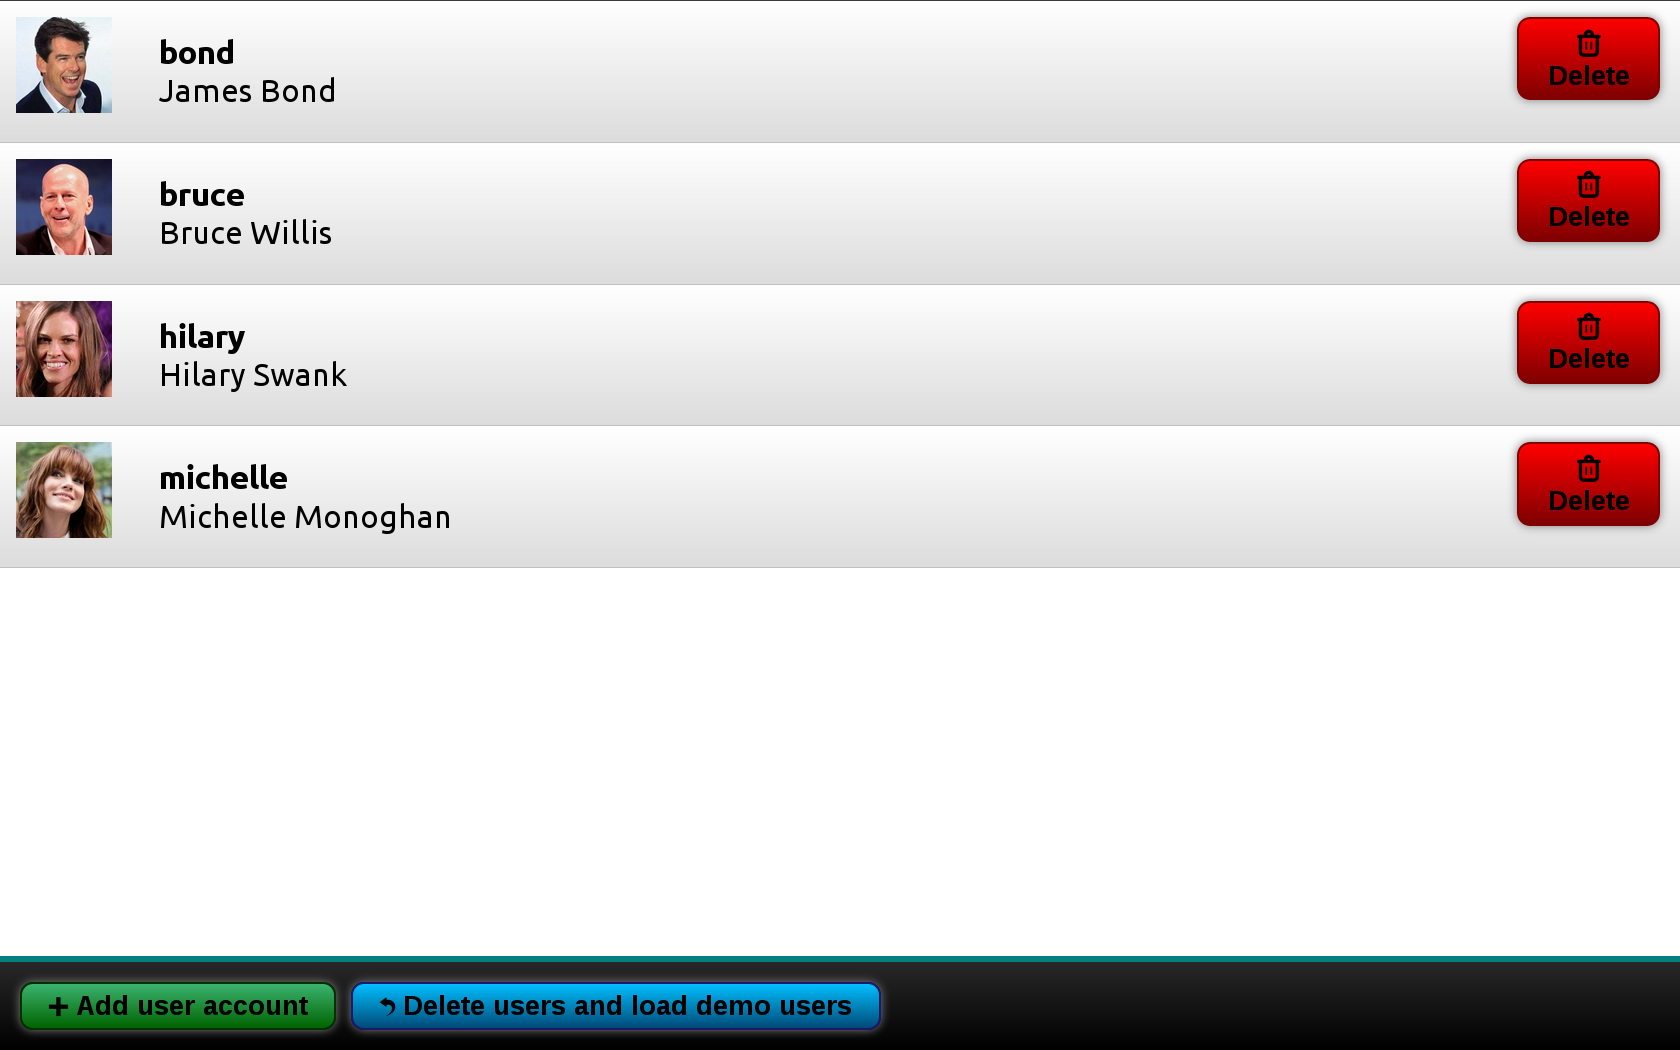
\includegraphics[height=0.325\textheight]{../ui/img/finalUi/accountView.png}
		\caption[Account screen]{Benutzer Verwaltung und Login Screen. Durch klick auf einen Benutzer kann sich der Benutzer mit dessen Konto anmelden.\\
		\license{cc by-sa 3.0 Gage Skidmore, cc by-sa 2.5 Rita Molnár, cc by-sa 3.0 Tabercil, cc by-sa 3.0 Manfred Werner}}
		\label{login screen}
	\end{figure}
	\begin{figure}[H]
		\centering
		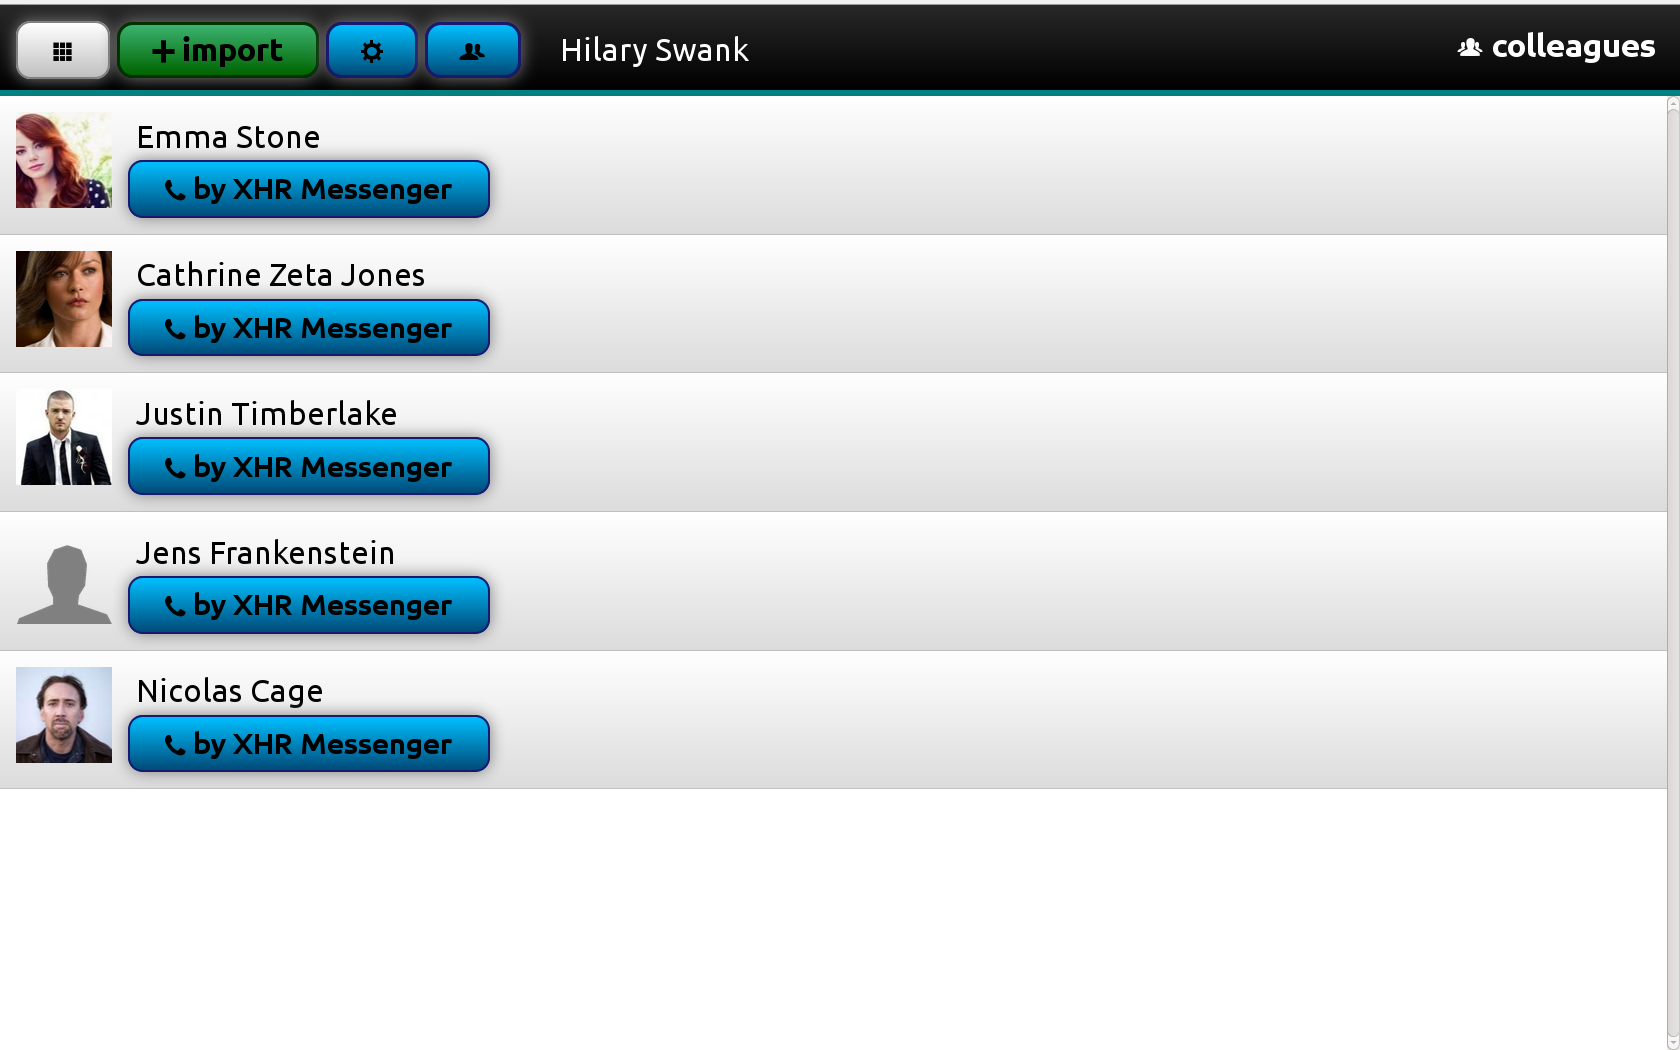
\includegraphics[height=0.325\textheight]{../ui/img/finalUi/contactView1.png}
		\caption[Contactbook screen]{Adressbuch: Von hier aus ruft der Benutzer seine Kontakte an. Die verschiedenen Adressbücher sind über das Listensymbol erreichbar.\\
		\license{cc by-sa 2.0 Gerald Geronimo, cc by 2.0 LeNair Xavier, modified by deerstop, cc by 3.0 Caroline Bonarde Ucci, cc by-sa 2.0 Nicolas Genin}}
		\label{contactbook screen}
	\end{figure}
	\begin{figure}[H]
		\centering
		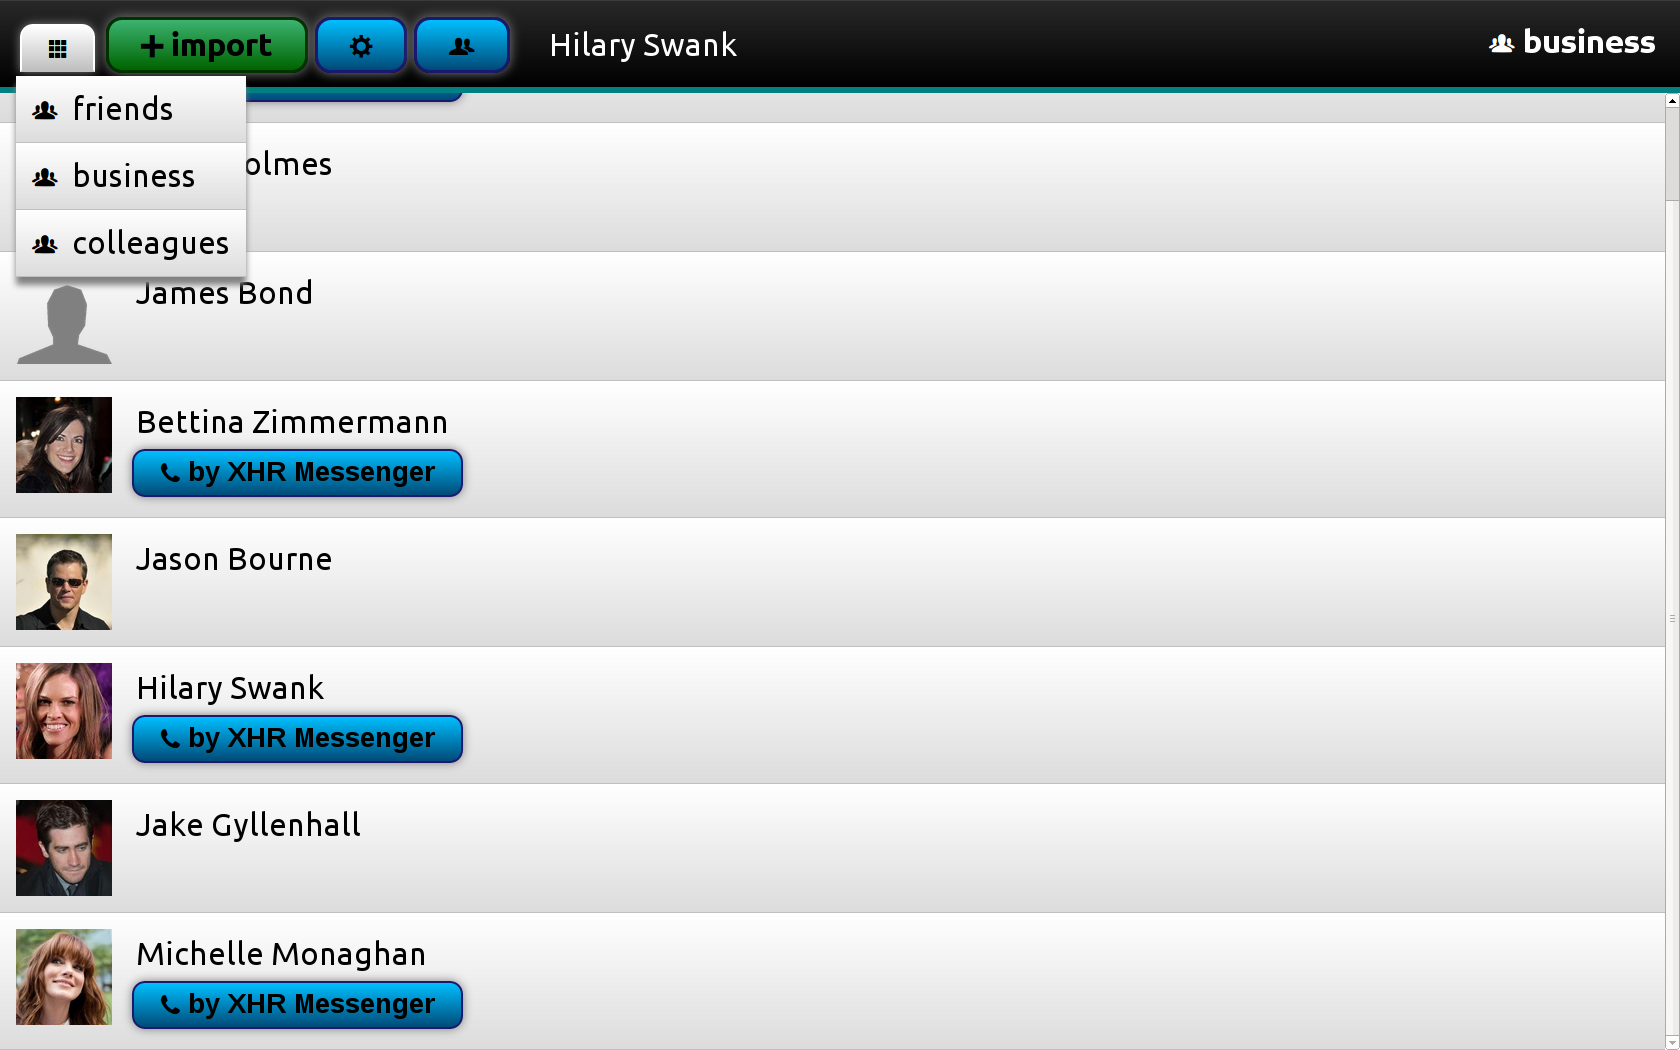
\includegraphics[height=0.4\textheight]{../ui/img/finalUi/contactView2.png}
		\caption[Contactbook list screen]{Auswahl des anzuzeigenden Adressbuches.\\
		\license{cc by 3.0 Siebbi, cc by-sa 2.0 Nicolas Genin, modified by CherryX, cc by-sa 3.0 Manfred Werner, cc by 3.0 Siebbi, cc by-sa 3.0 Tabercil}}
		\label{contactbook change}
	\end{figure}
	\begin{figure}[H]
		\centering
		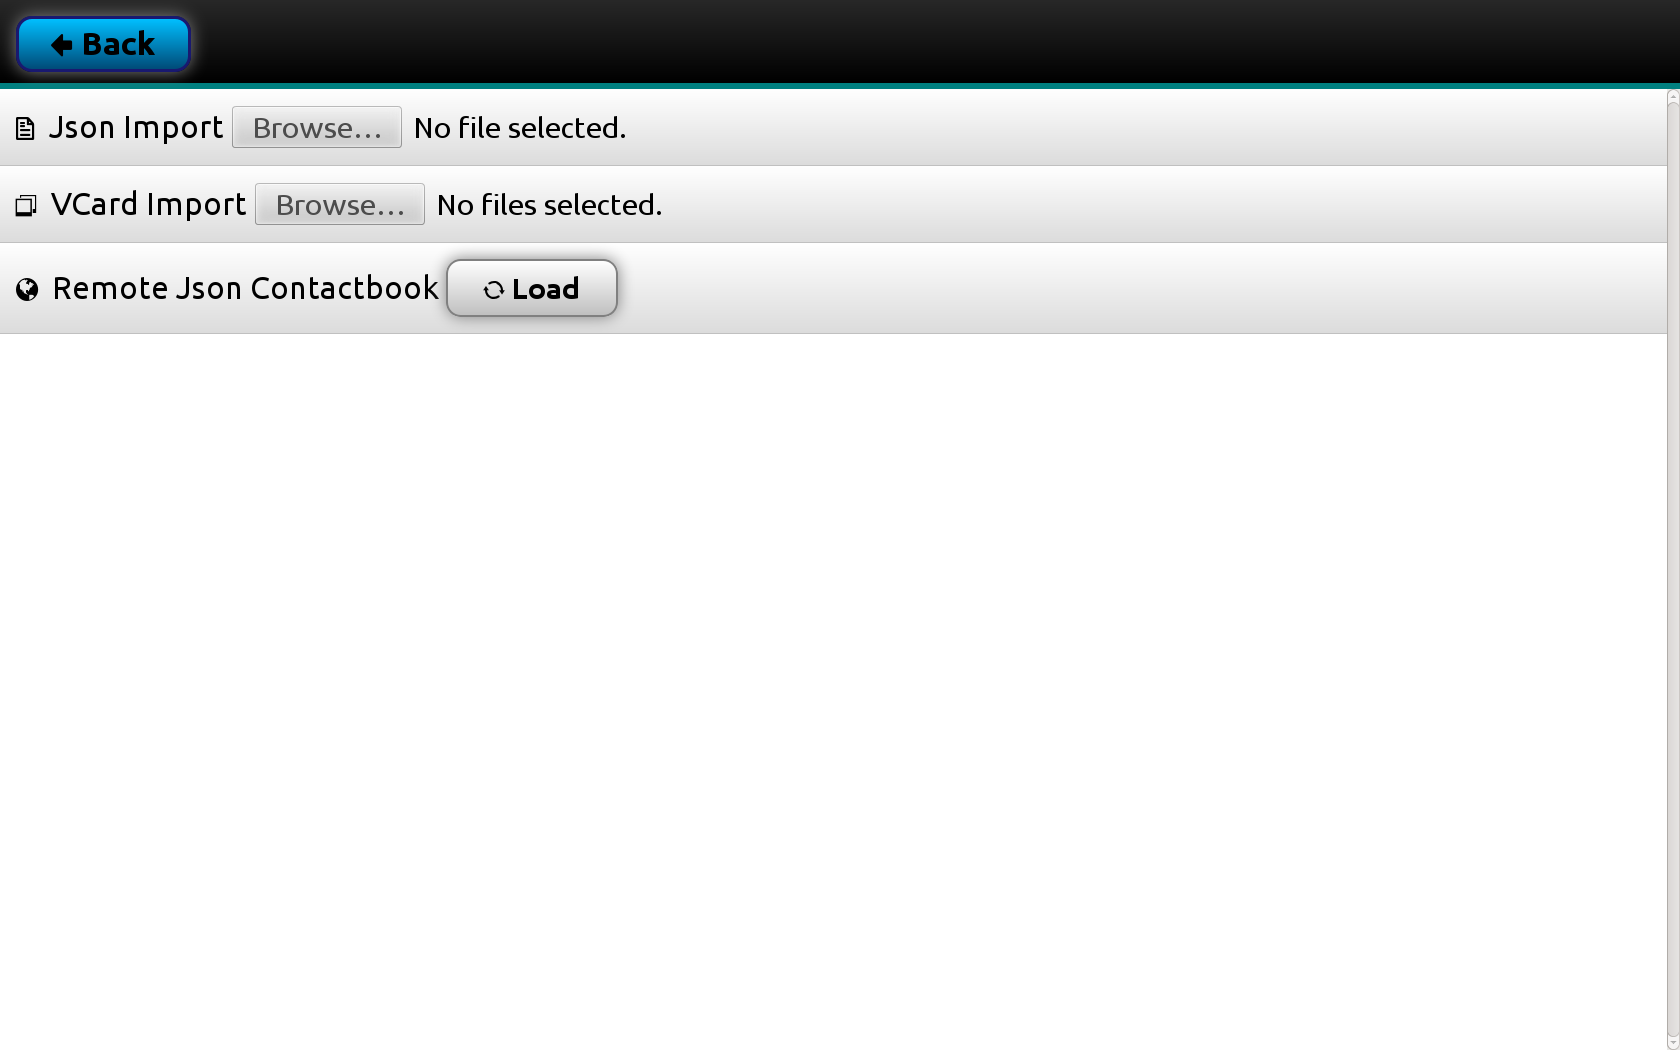
\includegraphics[height=0.4\textheight]{../ui/img/finalUi/importView.png}
		\caption[Contactbook import screen]{Adressbuch Import}
		\label{contactbook import screen}
	\end{figure}
	\begin{figure}[H]
		\centering
		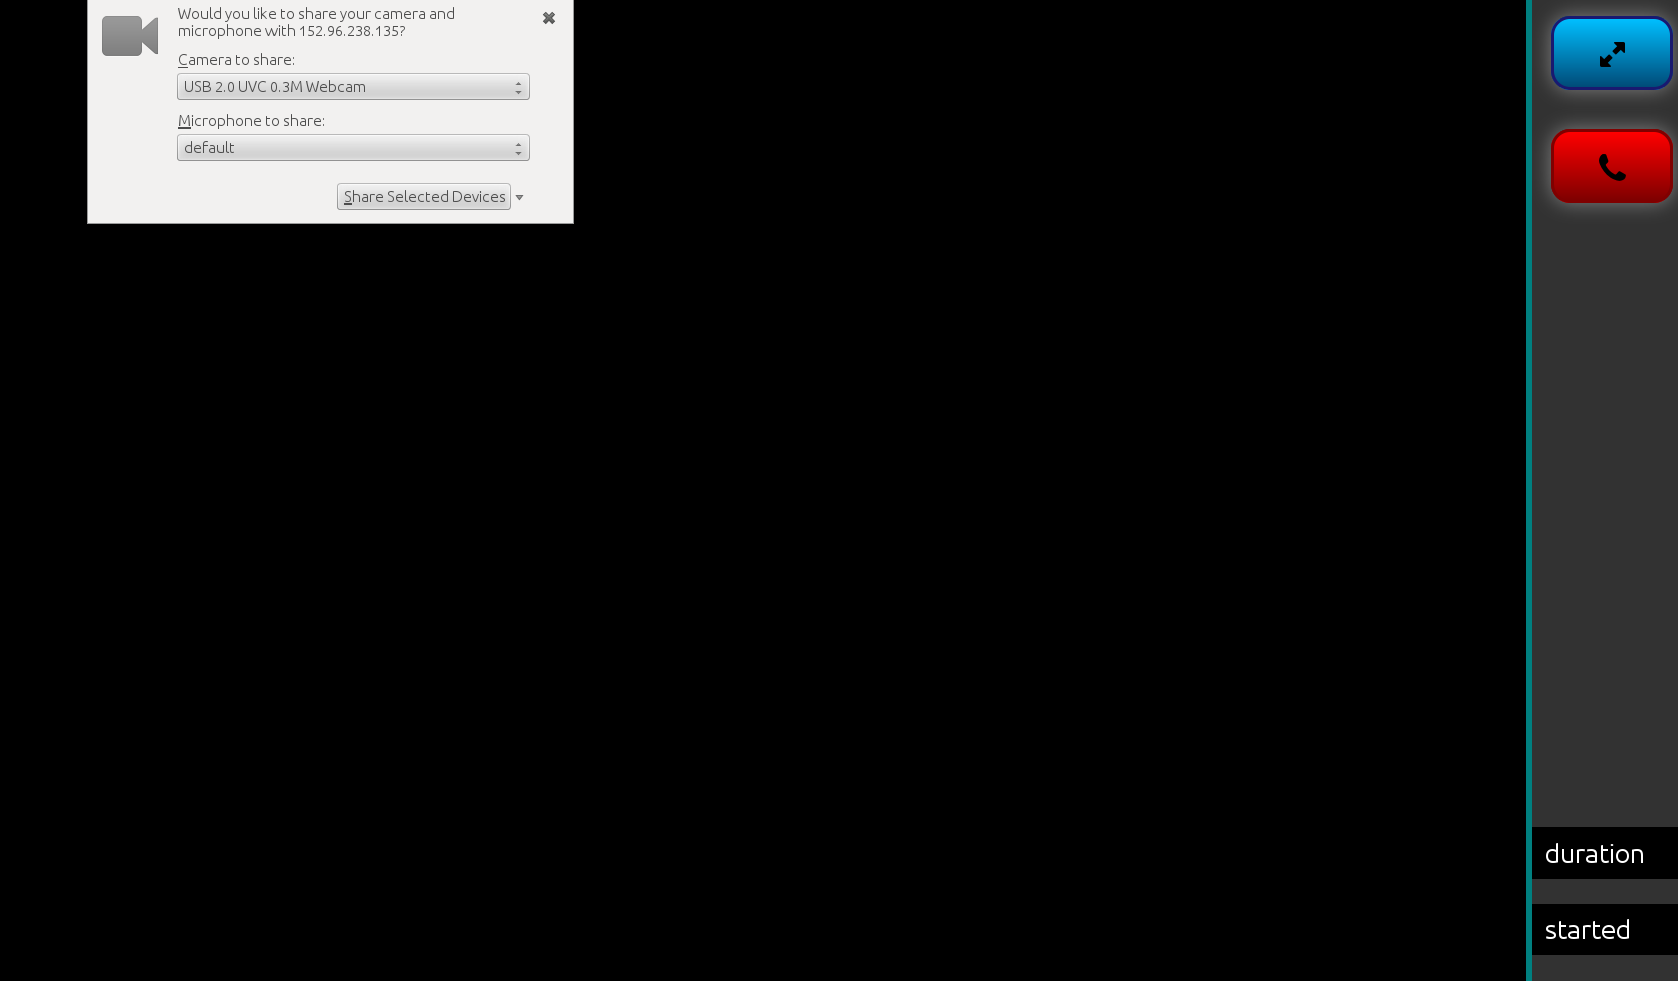
\includegraphics[height=0.4\textheight]{../ui/img/finalUi/cameraAccess.png}
		\caption[Camera access screen]{Anrufen: Kamerazugriff}
		\label{phone screen camera access}
	\end{figure}
	\begin{figure}[H]
		\centering
		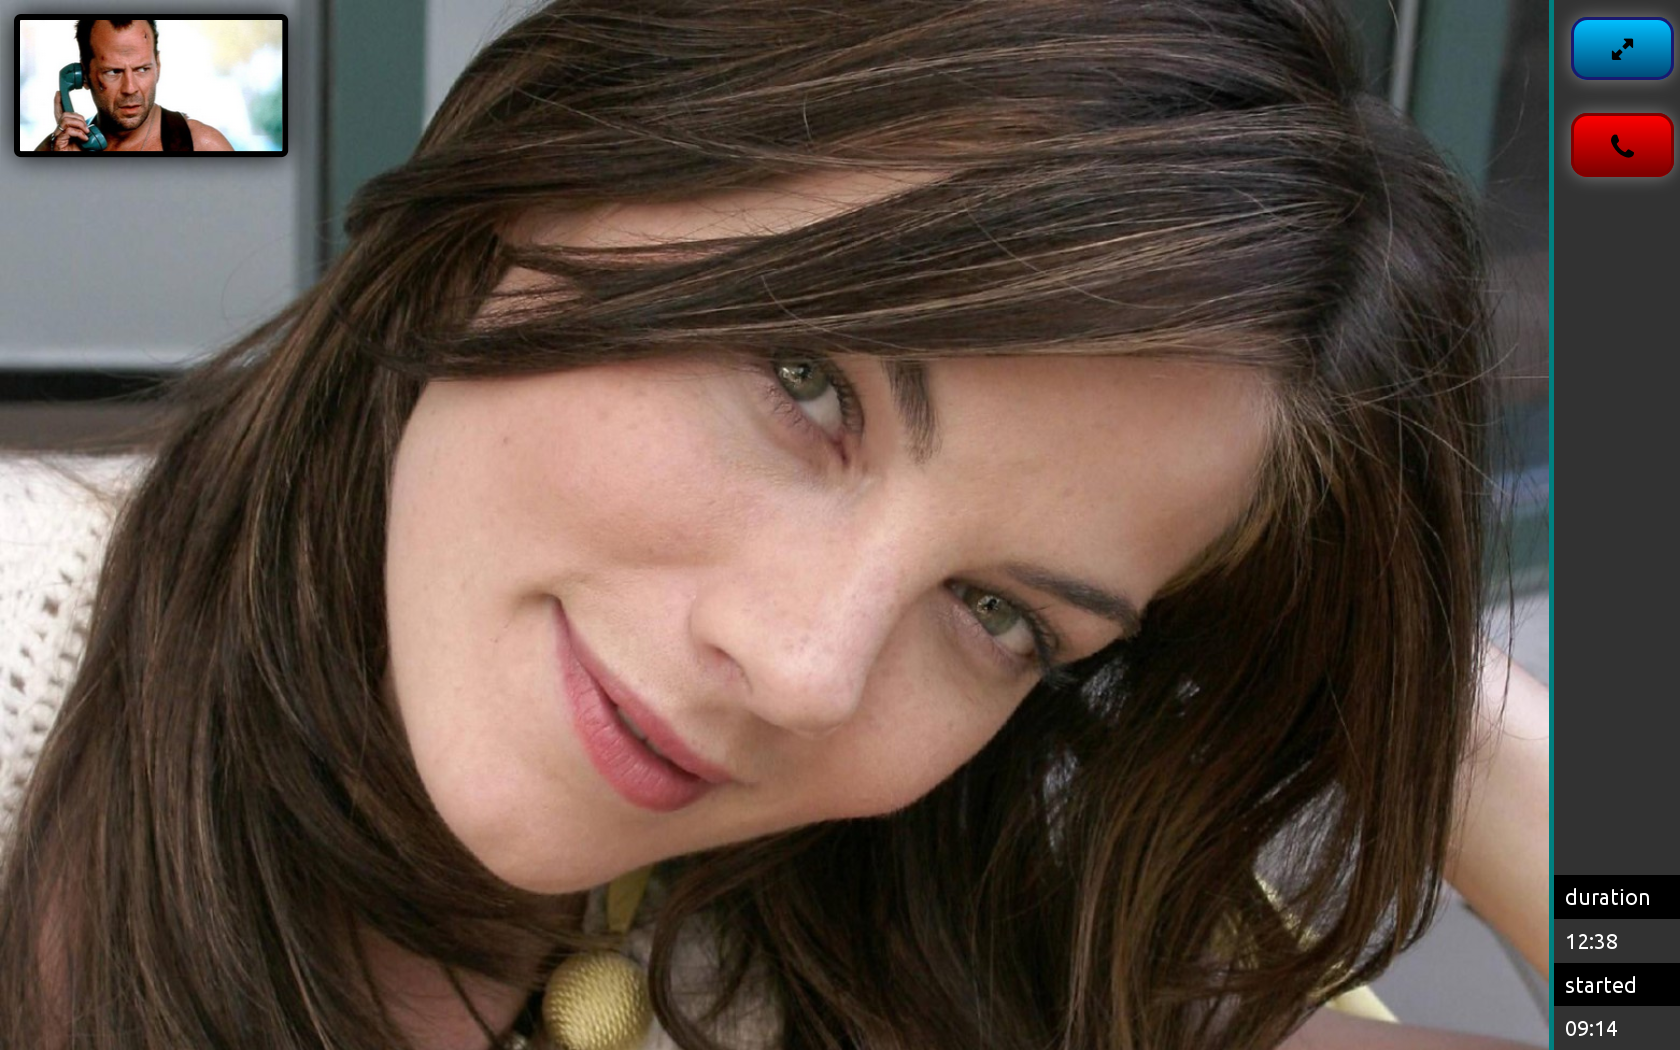
\includegraphics[height=0.4\textheight]{../ui/img/finalUi/phoneView.png}
		\caption[Call screen]{Anrufen}
		\label{phone screen}
	\end{figure}
	\begin{figure}[H]
		\centering
		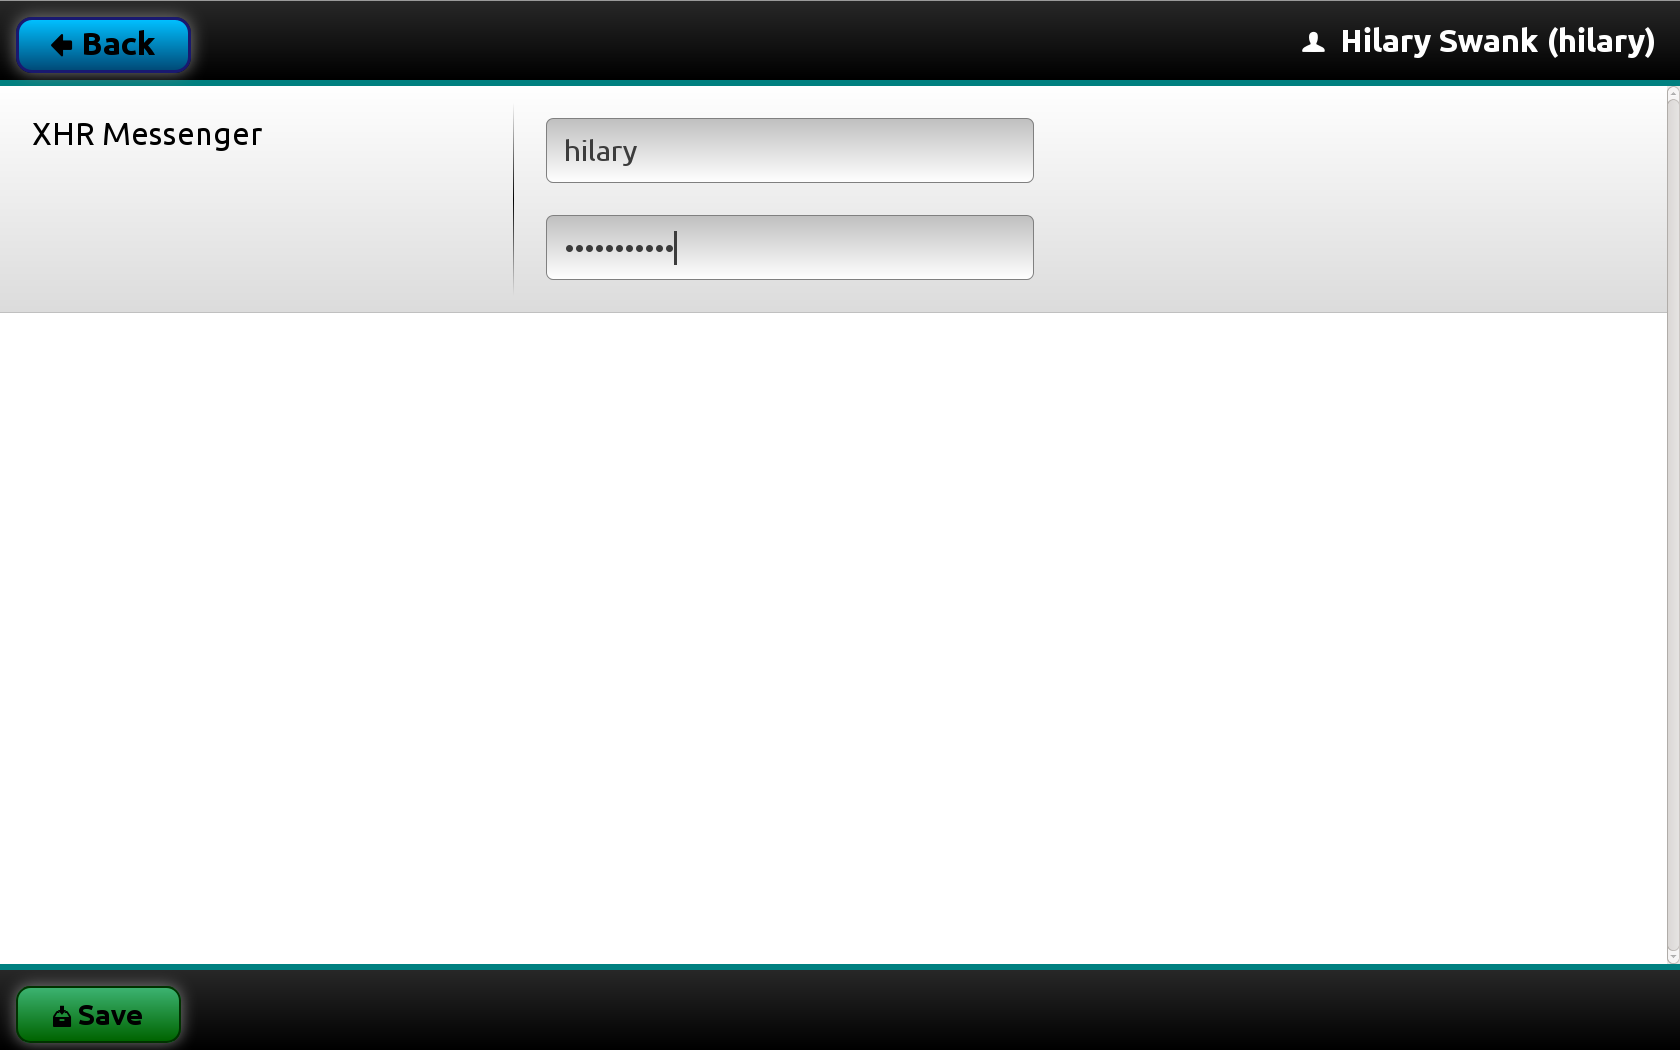
\includegraphics[height=0.4\textheight]{../ui/img/finalUi/accountEditView.png}
		\caption[Channel edit screen]{Account Setting: Verwaltung der Zugänge der aktiven Channels}
		\label{account edit screen}
	\end{figure}